
%% bare_jrnl.tex
%% V1.4
%% 2012/12/27
%% by Michael Shell
%% see http://www.michaelshell.org/
%% for current contact information.
%%
%% This is a skeleton file demonstrating the use of IEEEtran.cls
%% (requires IEEEtran.cls version 1.8 or later) with an IEEE journal paper.
%%
%% Support sites:
%% http://www.michaelshell.org/tex/ieeetran/
%% http://www.ctan.org/tex-archive/macros/latex/contrib/IEEEtran/
%% and
%% http://www.ieee.org/



% *** Authors should verify (and, if needed, correct) their LaTeX system  ***
% *** with the testflow diagnostic prior to trusting their LaTeX platform ***
% *** with production work. IEEE's font choices can trigger bugs that do  ***
% *** not appear when using other class files.                            ***
% The testflow support page is at:
% http://www.michaelshell.org/tex/testflow/


%%*************************************************************************
%% Legal Notice:
%% This code is offered as-is without any warranty either expressed or
%% implied; without even the implied warranty of MERCHANTABILITY or
%% FITNESS FOR A PARTICULAR PURPOSE! 
%% User assumes all risk.
%% In no event shall IEEE or any contributor to this code be liable for
%% any damages or losses, including, but not limited to, incidental,
%% consequential, or any other damages, resulting from the use or misuse
%% of any information contained here.
%%
%% All comments are the opinions of their respective authors and are not
%% necessarily endorsed by the IEEE.
%%
%% This work is distributed under the LaTeX Project Public License (LPPL)
%% ( http://www.latex-project.org/ ) version 1.3, and may be freely used,
%% distributed and modified. A copy of the LPPL, version 1.3, is included
%% in the base LaTeX documentation of all distributions of LaTeX released
%% 2003/12/01 or later.
%% Retain all contribution notices and credits.
%% ** Modified files should be clearly indicated as such, including  **
%% ** renaming them and changing author support contact information. **
%%
%% File list of work: IEEEtran.cls, IEEEtran_HOWTO.pdf, bare_adv.tex,
%%                    bare_conf.tex, bare_jrnl.tex, bare_jrnl_compsoc.tex,
%%                    bare_jrnl_transmag.tex
%%*************************************************************************

% Note that the a4paper option is mainly intended so that authors in
% countries using A4 can easily print to A4 and see how their papers will
% look in print - the typesetting of the document will not typically be
% affected with changes in paper size (but the bottom and side margins will).
% Use the testflow package mentioned above to verify correct handling of
% both paper sizes by the user's LaTeX system.
%
% Also note that the "draftcls" or "draftclsnofoot", not "draft", option
% should be used if it is desired that the figures are to be displayed in
% draft mode.
%
\documentclass[journal,onecolumn]{IEEEtran}
%
% If IEEEtran.cls has not been installed into the LaTeX system files,
% manually specify the path to it like:
% \documentclass[journal]{../sty/IEEEtran}





% Some very useful LaTeX packages include:
% (uncomment the ones you want to load)


% *** MISC UTILITY PACKAGES ***
%
%\usepackage{ifpdf}
% Heiko Oberdiek's ifpdf.sty is very useful if you need conditional
% compilation based on whether the output is pdf or dvi.
% usage:
% \ifpdf
%   % pdf code
% \else
%   % dvi code
% \fi
% The latest version of ifpdf.sty can be obtained from:
% http://www.ctan.org/tex-archive/macros/latex/contrib/oberdiek/
% Also, note that IEEEtran.cls V1.7 and later provides a builtin
% \ifCLASSINFOpdf conditional that works the same way.
% When switching from latex to pdflatex and vice-versa, the compiler may
% have to be run twice to clear warning/error messages.






% *** CITATION PACKAGES ***
%
%\usepackage{cite}
% cite.sty was written by Donald Arseneau
% V1.6 and later of IEEEtran pre-defines the format of the cite.sty package
% \cite{} output to follow that of IEEE. Loading the cite package will
% result in citation numbers being automatically sorted and properly
% "compressed/ranged". e.g., [1], [9], [2], [7], [5], [6] without using
% cite.sty will become [1], [2], [5]--[7], [9] using cite.sty. cite.sty's
% \cite will automatically add leading space, if needed. Use cite.sty's
% noadjust option (cite.sty V3.8 and later) if you want to turn this off
% such as if a citation ever needs to be enclosed in parenthesis.
% cite.sty is already installed on most LaTeX systems. Be sure and use
% version 4.0 (2003-05-27) and later if using hyperref.sty. cite.sty does
% not currently provide for hyperlinked citations.
% The latest version can be obtained at:
% http://www.ctan.org/tex-archive/macros/latex/contrib/cite/
% The documentation is contained in the cite.sty file itself.






% *** GRAPHICS RELATED PACKAGES ***
%
\usepackage{graphicx}
% declare the path(s) where your graphic files are
\graphicspath{{images/}}
% and their extensions so you won't have to specify these with
% every instance of \includegraphics
\DeclareGraphicsExtensions{.pdf,.jpeg,.png}
% graphicx was written by David Carlisle and Sebastian Rahtz. It is
% required if you want graphics, photos, etc. graphicx.sty is already
% installed on most LaTeX systems. The latest version and documentation
% can be obtained at: 
% http://www.ctan.org/tex-archive/macros/latex/required/graphics/
% Another good source of documentation is "Using Imported Graphics in
% LaTeX2e" by Keith Reckdahl which can be found at:
% http://www.ctan.org/tex-archive/info/epslatex/
%
% latex, and pdflatex in dvi mode, support graphics in encapsulated
% postscript (.eps) format. pdflatex in pdf mode supports graphics
% in .pdf, .jpeg, .png and .mps (metapost) formats. Users should ensure
% that all non-photo figures use a vector format (.eps, .pdf, .mps) and
% not a bitmapped formats (.jpeg, .png). IEEE frowns on bitmapped formats
% which can result in "jaggedy"/blurry rendering of lines and letters as
% well as large increases in file sizes.
%
% You can find documentation about the pdfTeX application at:
% http://www.tug.org/applications/pdftex





% *** MATH PACKAGES ***
%
%\usepackage[cmex10]{amsmath}
% A popular package from the American Mathematical Society that provides
% many useful and powerful commands for dealing with mathematics. If using
% it, be sure to load this package with the cmex10 option to ensure that
% only type 1 fonts will utilized at all point sizes. Without this option,
% it is possible that some math symbols, particularly those within
% footnotes, will be rendered in bitmap form which will result in a
% document that can not be IEEE Xplore compliant!
%
% Also, note that the amsmath package sets \interdisplaylinepenalty to 10000
% thus preventing page breaks from occurring within multiline equations. Use:
%\interdisplaylinepenalty=2500
% after loading amsmath to restore such page breaks as IEEEtran.cls normally
% does. amsmath.sty is already installed on most LaTeX systems. The latest
% version and documentation can be obtained at:
% http://www.ctan.org/tex-archive/macros/latex/required/amslatex/math/





% *** SPECIALIZED LIST PACKAGES ***
%
%\usepackage{algorithmic}
% algorithmic.sty was written by Peter Williams and Rogerio Brito.
% This package provides an algorithmic environment fo describing algorithms.
% You can use the algorithmic environment in-text or within a figure
% environment to provide for a floating algorithm. Do NOT use the algorithm
% floating environment provided by algorithm.sty (by the same authors) or
% algorithm2e.sty (by Christophe Fiorio) as IEEE does not use dedicated
% algorithm float types and packages that provide these will not provide
% correct IEEE style captions. The latest version and documentation of
% algorithmic.sty can be obtained at:
% http://www.ctan.org/tex-archive/macros/latex/contrib/algorithms/
% There is also a support site at:
% http://algorithms.berlios.de/index.html
% Also of interest may be the (relatively newer and more customizable)
% algorithmicx.sty package by Szasz Janos:
% http://www.ctan.org/tex-archive/macros/latex/contrib/algorithmicx/




% *** ALIGNMENT PACKAGES ***
%
%\usepackage{array}
% Frank Mittelbach's and David Carlisle's array.sty patches and improves
% the standard LaTeX2e array and tabular environments to provide better
% appearance and additional user controls. As the default LaTeX2e table
% generation code is lacking to the point of almost being broken with
% respect to the quality of the end results, all users are strongly
% advised to use an enhanced (at the very least that provided by array.sty)
% set of table tools. array.sty is already installed on most systems. The
% latest version and documentation can be obtained at:
% http://www.ctan.org/tex-archive/macros/latex/required/tools/
\usepackage{float}


% IEEEtran contains the IEEEeqnarray family of commands that can be used to
% generate multiline equations as well as matrices, tables, etc., of high
% quality.




% *** SUBFIGURE PACKAGES ***
\ifCLASSOPTIONcompsoc
  \usepackage[caption=false,font=normalsize,labelfont=sf,textfont=sf]{subfig}
\else
  \usepackage[caption=false,font=footnotesize]{subfig}
\fi
% subfig.sty, written by Steven Douglas Cochran, is the modern replacement
% for subfigure.sty, the latter of which is no longer maintained and is
% incompatible with some LaTeX packages including fixltx2e. However,
% subfig.sty requires and automatically loads Axel Sommerfeldt's caption.sty
% which will override IEEEtran.cls' handling of captions and this will result
% in non-IEEE style figure/table captions. To prevent this problem, be sure
% and invoke subfig.sty's "caption=false" package option (available since
% subfig.sty version 1.3, 2005/06/28) as this is will preserve IEEEtran.cls
% handling of captions.
% Note that the Computer Society format requires a larger sans serif font
% than the serif footnote size font used in traditional IEEE formatting
% and thus the need to invoke different subfig.sty package options depending
% on whether compsoc mode has been enabled.
%
% The latest version and documentation of subfig.sty can be obtained at:
% http://www.ctan.org/tex-archive/macros/latex/contrib/subfig/




% *** FLOAT PACKAGES ***
%
%\usepackage{fixltx2e}
% fixltx2e, the successor to the earlier fix2col.sty, was written by
% Frank Mittelbach and David Carlisle. This package corrects a few problems
% in the LaTeX2e kernel, the most notable of which is that in current
% LaTeX2e releases, the ordering of single and double column floats is not
% guaranteed to be preserved. Thus, an unpatched LaTeX2e can allow a
% single column figure to be placed prior to an earlier double column
% figure. The latest version and documentation can be found at:
% http://www.ctan.org/tex-archive/macros/latex/base/


%\usepackage{stfloats}
% stfloats.sty was written by Sigitas Tolusis. This package gives LaTeX2e
% the ability to do double column floats at the bottom of the page as well
% as the top. (e.g., "\begin{figure*}[!b]" is not normally possible in
% LaTeX2e). It also provides a command:
%\fnbelowfloat
% to enable the placement of footnotes below bottom floats (the standard
% LaTeX2e kernel puts them above bottom floats). This is an invasive package
% which rewrites many portions of the LaTeX2e float routines. It may not work
% with other packages that modify the LaTeX2e float routines. The latest
% version and documentation can be obtained at:
% http://www.ctan.org/tex-archive/macros/latex/contrib/sttools/
% Do not use the stfloats baselinefloat ability as IEEE does not allow
% \baselineskip to stretch. Authors submitting work to the IEEE should note
% that IEEE rarely uses double column equations and that authors should try
% to avoid such use. Do not be tempted to use the cuted.sty or midfloat.sty
% packages (also by Sigitas Tolusis) as IEEE does not format its papers in
% such ways.
% Do not attempt to use stfloats with fixltx2e as they are incompatible.
% Instead, use Morten Hogholm'a dblfloatfix which combines the features
% of both fixltx2e and stfloats:
%
% \usepackage{dblfloatfix}
% The latest version can be found at:
% http://www.ctan.org/tex-archive/macros/latex/contrib/dblfloatfix/




%\ifCLASSOPTIONcaptionsoff
%  \usepackage[nomarkers]{endfloat}
% \let\MYoriglatexcaption\caption
% \renewcommand{\caption}[2][\relax]{\MYoriglatexcaption[#2]{#2}}
%\fi
% endfloat.sty was written by James Darrell McCauley, Jeff Goldberg and 
% Axel Sommerfeldt. This package may be useful when used in conjunction with 
% IEEEtran.cls'  captionsoff option. Some IEEE journals/societies require that
% submissions have lists of figures/tables at the end of the paper and that
% figures/tables without any captions are placed on a page by themselves at
% the end of the document. If needed, the draftcls IEEEtran class option or
% \CLASSINPUTbaselinestretch interface can be used to increase the line
% spacing as well. Be sure and use the nomarkers option of endfloat to
% prevent endfloat from "marking" where the figures would have been placed
% in the text. The two hack lines of code above are a slight modification of
% that suggested by in the endfloat docs (section 8.4.1) to ensure that
% the full captions always appear in the list of figures/tables - even if
% the user used the short optional argument of \caption[]{}.
% IEEE papers do not typically make use of \caption[]'s optional argument,
% so this should not be an issue. A similar trick can be used to disable
% captions of packages such as subfig.sty that lack options to turn off
% the subcaptions:
% For subfig.sty:
% \let\MYorigsubfloat\subfloat
% \renewcommand{\subfloat}[2][\relax]{\MYorigsubfloat[]{#2}}
% However, the above trick will not work if both optional arguments of
% the \subfloat command are used. Furthermore, there needs to be a
% description of each subfigure *somewhere* and endfloat does not add
% subfigure captions to its list of figures. Thus, the best approach is to
% avoid the use of subfigure captions (many IEEE journals avoid them anyway)
% and instead reference/explain all the subfigures within the main caption.
% The latest version of endfloat.sty and its documentation can obtained at:
% http://www.ctan.org/tex-archive/macros/latex/contrib/endfloat/
%
% The IEEEtran \ifCLASSOPTIONcaptionsoff conditional can also be used
% later in the document, say, to conditionally put the References on a 
% page by themselves.




% *** PDF, URL AND HYPERLINK PACKAGES ***
%
%\usepackage{url}
% url.sty was written by Donald Arseneau. It provides better support for
% handling and breaking URLs. url.sty is already installed on most LaTeX
% systems. The latest version and documentation can be obtained at:
% http://www.ctan.org/tex-archive/macros/latex/contrib/url/
% Basically, \url{my_url_here}.




% *** Do not adjust lengths that control margins, column widths, etc. ***
% *** Do not use packages that alter fonts (such as pslatex).         ***
% There should be no need to do such things with IEEEtran.cls V1.6 and later.
% (Unless specifically asked to do so by the journal or conference you plan
% to submit to, of course. )


% correct bad hyphenation here
\hyphenation{op-tical net-works semi-conduc-tor}


\begin{document}

\title{A Biologically Plausable Neurodynamical \\ Model of Color \& Form \\ in the Primary Visual Cortex}
%
%
% author names and IEEE memberships
% note positions of commas and nonbreaking spaces ( ~ ) LaTeX will not break
% a structure at a ~ so this keeps an author's name from being broken across
% two lines.
% use \thanks{} to gain access to the first footnote area
% a separate \thanks must be used for each paragraph as LaTeX2e's \thanks
% was not built to handle multiple paragraphs
%

\author{Sean Thomas Connolly% <-this % stops a space
\thanks{Author: Sean Thomas Connolly, connolly.st@gmail.com}% <-this % stops a space
\thanks{Advisor: Xavier Otazu,  Computer Vision Center, Computer Science Department, Universitat Autònoma de Barcelona, Barcelona, Spain }% <-this % stops a space% stops a space
\thanks{Submitted: September 2014}}

% note the % following the last \IEEEmembership and also \thanks - 
% these prevent an unwanted space from occurring between the last author name
% and the end of the author line. i.e., if you had this:
% 
% \author{....lastname \thanks{...} \thanks{...} }
%                     ^------------^------------^----Do not want these spaces!
%
% a space would be appended to the last name and could cause every name on that
% line to be shifted left slightly. This is one of those "LaTeX things". For
% instance, "\textbf{A} \textbf{B}" will typeset as "A B" not "AB". To get
% "AB" then you have to do: "\textbf{A}\textbf{B}"
% \thanks is no different in this regard, so shield the last } of each \thanks
% that ends a line with a % and do not let a space in before the next \thanks.
% Spaces after \IEEEmembership other than the last one are OK (and needed) as
% you are supposed to have spaces between the names. For what it is worth,
% this is a minor point as most people would not even notice if the said evil
% space somehow managed to creep in.



% The paper headers
\markboth{Master Thesis Dissertation, Master in Computer Vision, July 2014}%
{Shell \MakeLowercase{\textit{et al.}}: Bare Demo of IEEEtran.cls for Journals}
% The only time the second header will appear is for the odd numbered pages
% after the title page when using the twoside option.



% make the title area
\maketitle

% As a general rule, do not put math, special symbols or citations
% in the abstract or keywords.
\begin{abstract}
We present a computational model of the primary visual cortex (V1) inspired by current neurobiological understanding. This understanding treats color and shape as intrinsically connected and, as a consequence, predicts perceptual phenomena such as color induction and assimilation to arise very early in visual processing. We incorporate this understanding into a dynamical model of neuronal activity responding to static or dynamic visual stimuli. Our model confirms the psychophysical predictions on a range of experiments, offering credence to the biological theories.
% TODO Should we end with a statement of possible applications (e.g.: data preprocessing)?
\end{abstract}

% Note that keywords are not normally used for peerreview papers.
\begin{IEEEkeywords}
primary visual cortex, striate cortex, V1, receptive field, single opponent, double opponent, color assimilation, color induction
\end{IEEEkeywords}


% For peer review papers, you can put extra information on the cover
% page as needed:
% \ifCLASSOPTIONpeerreview
% \begin{center} \bfseries EDICS Category: 3-BBND \end{center}
% \fi
%
% For peerreview papers, this IEEEtran command inserts a page break and
% creates the second title. It will be ignored for other modes.
\IEEEpeerreviewmaketitle



\section{Introduction}

% TODO perhaps the distinction between physical color and perception color is valuable here?

\IEEEPARstart{C}{olor} induction and contrast are two related, opposing, perceptual phenomena. The former is a change in perceived color "toward" a nearby color, while the latter is a change of one color "away" from the nearby color. Neurophysiological research suggests that these phenomena may arise as early in primate vision as the primary visual cortex (V1). It is proposed that the boundaries between two colored regions drive these effects. Specifically, research in the field describes neurons which fire selectively to boundaries between certain colors, so called double opponent cells, and identifies them as being critically related to the color perceived.

Within, we propose a computational model designed around the current understanding of this biology. We present two implementations, one more biologically accurate, and another more computationally elegant. We explore the behavior of these models with respect to what they can teach us about the assumed biological theories, as well as their application to the field of computer vision.


%%%%%%%%%%%%%%%%%%%%%%%%%%%%%%%%%%%%%%%%%%%%%%%%%%%%%%%%%%%%%%%%
%
% STATE OF THE ART
%
% A bibliographic review on of the problem topic.
%
%%%%%%%%%%%%%%%%%%%%%%%%%%%%%%%%%%%%%%%%%%%%%%%%%%%%%%%%%%%%%%%%
\section{State of the art}


\subsection{Neurobiology}

Historically, it was widely believed that color and shape are two distinct aspects of visual perception. Truly, this line of though is intuitive: one can perceive the color of a flat surface which occupies our full field of vision, despite its lack of 'shape', likewise we can see the shape of achromatic objects, as in black and white film. This theory of perception innervated neurophysiological understanding and was supported by neurobiological findings, such as that the lateral geniculate nucleus (LGN), the pathway which carries information from the retina to the primary visual cortex (V1), consists of three entirely distinct layers; two (the parvicellular and konicellular) carrying only color information, and one (the magnocellular) dealing purely in achromatic contrast (edge) information. Based on early anatomical observations, it was proposed that these three LGN pathways for color and contrast are then processed into two separate streams in V1, one for color and the other for form. This separate handling of color and form indicated to researchers that, as suspected, these two perceptual concepts are, indeed, processed separately in the brain.


Research in the past decade or so has seen a shift from this thinking, however. Psychophysical observations, such as those in Figure \ref{fig:blur-effect}, influenced researchers to consider that color and form are more intrinsically related than previously thought. In these examples, we see that the \textit{perceived} color of the inner square is highly dependent on the background and, most importantly, how the inner square \textit{contacts} the background. The color perceived is not just determined by the physical properties of the surface, but also by the context in which the surface is viewed. Furthermore, we can observe that this contextual influence comes largely from the boundary edges of the surface: in example (c), the dulling color assimilation effect witnessed in (b) is almost entirely negated by simply adding a thin border. That is, by removing contact between the inner square and the background, the effect of the context is significantly reduced. In fact, "the color appearance of a region may be more dependent on color contrast at the boundary of the region than it is on the spectral reflectance of the region's interior." \cite[p.572]{chualupa:encyclopedia}

\begin{figure}[H]
    \centering
    \subfloat[] {
\includegraphics[width=100pt]{example_1a}}
    ~
    \subfloat[] {
\includegraphics[width=100pt]{example_1b}}
    ~
    \subfloat[] {
\includegraphics[width=100pt]{example_1c}}
    ~
    \subfloat[] {
\includegraphics[width=100pt]{example_1d}}
    \caption{Psychophysical example emphasizing the effect of edge contrast in color perception. In all cases, the center square is the same physical color. On (a) the green background, however, it appears much brighter than it does on (b) the red background. (c) Adding a thin black border negates the assimilation effect, increasing the perceived brightness of the center square. (d) Blurring the background, on the other hand, seems to enhance assimilation, lowering the perceived brightness at the center.}
    \label{fig:blur-effect}
\end{figure}

With these psychophysical observations in mind, much research has been focused on the specific neurobiological mechanisms behind the perception of color. The current view holds that while the LGN does indeed carry color and contrast information through distinct pathways to the striate cortex (V1), once there, it is now thought that color and form become deeply intertwined as they are processed further.

To explain the simultaneous processing of color and form in V1, the literature proposes two broad classifications of neurons: single opponent cells, \& double opponent cells (Johnson et al. Color and Orientation in V1). Opponency, in neurobiology, refers to antagonistic inputs to a neuron: one source of input exciting the neuron, while another source inhibits it. If the two sources provide equal input, for example, they would cancel out and the neuron would not fire. With respect to cells in the early visual system, we are here specifically referring to chromatic and spatial opponency, as will be detailed below. Briefly, single opponent cells respond best to large areas of color, while double opponent cells respond only to the boundaries between such areas.


\subsection*{Single Opponent Neurons}

Single opponent neurons are built using the classical center/surround receptive fields. The ON receptive field exciting the cell when presented with a particular color in the center, the OFF receptive field exciting the cell when another color is \textit{removed} from the surround.


\textbf{// TODO} \textit{add image of simple behavior: gradient response to isoluminant chromatic boundary}

\textbf{// TODO} \textit{add image of simple behavior: no response to intensity changes}

\begin{figure}[H]
    \subfloat[Symmetric Balanced]  {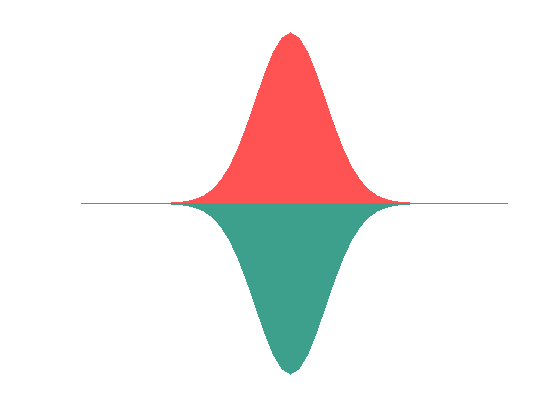
\includegraphics[width=160pt]{rf_so_1}}
    \subfloat[Symmetric Unbalanced]{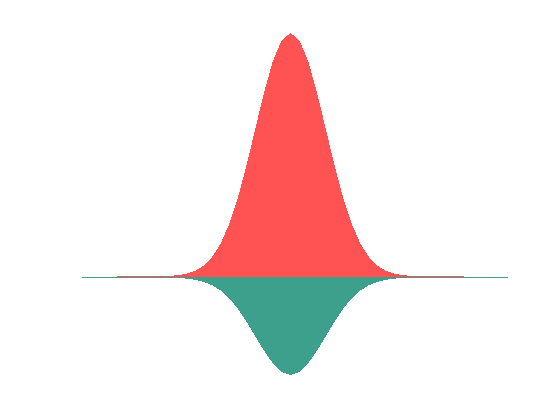
\includegraphics[width=160pt]{rf_so_2}}
    \subfloat[Center/Surround]     {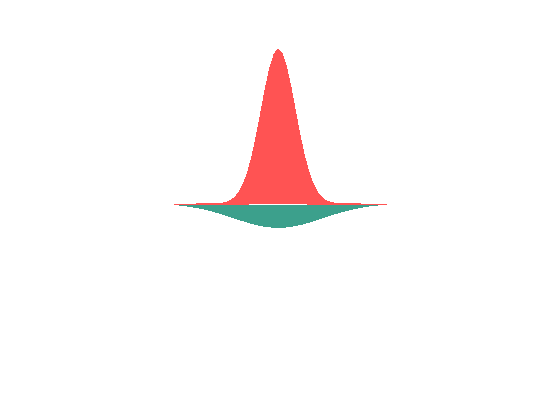
\includegraphics[width=160pt]{rf_so_3}}
    \caption{Visualization of a variety of single opponent (SO) receptive fields.}
    \label{fig:rf-so}
\end{figure}

\subsubsection*{Achromatic Single Opponent Neurons}

Sometimes called non-opponent cells, they have no chromatic nor spatial opponency. Instead, they amalgamate all color input in a balanced manner so as to only respond to changes in luminosity. Technically, we can consider non-opponent cells to be a special case of single opponent cells.

\textbf{// TODO} are NO cells the same as SO cells? What about achromatic single opponent cells?

\textbf{// TODO} \textit{add image depicting example receptive field(s)}

\textbf{// TODO} \textit{add image of simple behavior: gradient response to ((mono)chromatic) intensity changes}

\textbf{// TODO} \textit{add image of simple behavior: no response to isoluminant chromatic boundaries}

\subsection*{Double Opponent Neurons}

\textbf{Point:}
Double opponent neurons are edge detectors. 

\textbf{Story:}
Double opponent neurons are a topic of confusion in the field of neurobiology. All researchers on the topic seem to agree that the input to the neuron is that of two single opponent neurons itself. In this sense, the term "double opponent" can be thought of as indicating that the dimensionality of color opponency has been doubled. However, another camp of researchers take the definition a step further and suggest that the two SO inputs are spatially offset. By this definition, the term "double opponent" is thought to indicate that the cell is sensitive to opponency in two \textit{different} dimensions, color and space.

The distinction is non-trivial as the response patterns differ, and thus the interpretation of their role in vision differs.

\textbf{// TODO} \textbf{present the differences between the two DO configurations}

\begin{figure}[H]
    \subfloat[Symmetric Balanced]  {
\includegraphics[width=160pt]{rf_do_1}}
    \subfloat[Symmetric Unbalanced]{
\includegraphics[width=160pt]{rf_do_2}}
    \subfloat[Center/Surround]     {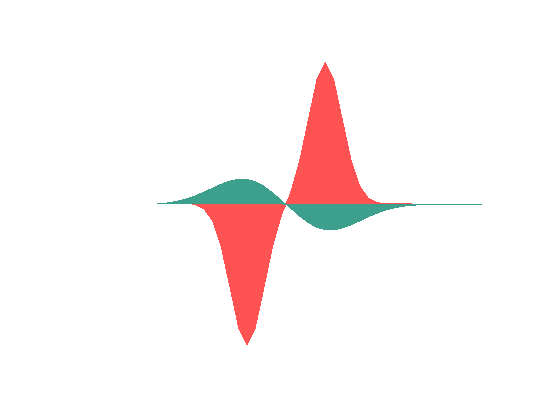
\includegraphics[width=160pt]{rf_do_4}}
    \caption{Visualization of a variety of double opponent (DO) receptive fields.}
    \label{fig:rf-do}
\end{figure}

\subsubsection*{Orientation Selectivity}

Research shows that cells identified as double opponent are orientation selective. That is, they respond most strongly when stimulated by a border of particular orientation, less so with variation from that preferred orientation, and weekly, if at all, to borders orthogonal to the preferred orientation. This is intuitive given the organization of the receptive field as previously defined.

\textbf{// TODO} \textbf{describe Orientation Selectivity}

\textbf{// TODO} \textit{add image depicting example receptive field(s)}

\textbf{// TODO} \textit{add image of simple behavior: peak activity AT sharp edge}


\subsubsection*{Spatial Frequency Selectivity}

It is recognized that


\subsubsection*{Achromatic Double Opponent Neurons}

\textbf{// TODO} \textbf{describe achromatic double opponent cells}



\textbf{// TODO} \textit{add image of Shapley response curves for NO, SO, \& DO}

\textbf{// TODO} \textit{mention relative abundance of NO, SO, \& DO}

To recapitulate: non-opponent neurons have no color preferences and fire equally to chromatic or achromatic luminosity changes, single opponent neurons are color preferring and fire best to full field stimulation, and double opponent neurons are color preferring but fire only at the boundaries between particular colors.


\subsection{Computational Modeling:}

This model is an extension of that presented by Penacchio \textit{et al.} \cite{otazu:plosone}, itself based on work by Z. Li \cite{li:1998, li:1999}. Before describing our implementation, it is important to review prior art. As our goal is to model the behavior of non-opponent, single opponent, and double opponent cells, we will also review other computational endeavors approaching the issue of color and form from a biologically inspired perspective.


\subsection*{Li's Neurodynamical Model for Segmentation (1999)}
In Li's original work, a neurodynamical model was presented which focused on the issue of region segmentation using local interactions between neurons. In the interest of simplicity, Li's implementation dealt only with the nature of these interactions and the signal processing which emerges, ignoring where the data might come from. Conceptually, Li defined neurons by the physical position in the image and the 'feature' to which they are sensitive. She then defined the connections between these neurons such that those physically close to each other, and sensitive to similar features, interacted most strongly.

In the model presented, Li used oriented bars as features, though expressed that any logical feature could be reasonably considered in its place. This choice was biologically inspired by neurons sensitive to specifically oriented bars. When considering such features, inter-neuronal connections can be logically deduced: two neurons positively interact most when both are sensitive to similarly oriented bars and are co-located along that same orientation. Two neurons negatively interact most when either of these two conditions is not met.

By defining the neuronal connectivity in this manner, neurons sensitive to co-located and co-aligned bars positively interact with each other to enhance their collective response to the stimuli. From these local interactions, global features are enhanced if they satisfy the neuronal connectivity rules. Li showed that this method can be used to identify boundaries between regions for which normal segmentation methods struggle.

\begin{itemize}
    \item No color, just black \& white \textit{lines}
    \item No sense of scales
    \item Dynamical processing
\end{itemize}


\subsection*{Penacchio, Otazu, \& Dempere-Marco's Neurodynamical Model for Brightness Induction (2013)}
Li's work laid the foundation for Penacchio \textit{et al.} who extended the model to a usable framework which:
\begin{enumerate}
    \item Uses real black \& white images /movies as input.
    \item Utilizes discrete wavelet transforms to extract edges (more on this later).
    \item Added multi scale support.
    \item Summarizes the results into an output 'perceptual image'.
\end{enumerate}
Their research was focused on observing brightness induction (BI) arising from such a neurodynamical model.
\begin{itemize}
    \item No color, just black \& white \textit{edges}
    \item Generalized to real images (edges vs lines)
    \item Added scales
    \item Dynamical processing
    \item \textbf{Avoid detail, save that for \textit{Method}..?}
    \item Extension of Z. Li's edge detection work
    \item Uses DWT to extract oriented edges in grayscale
    \begin{itemize}
        \item ..in our context, it's essentially a luminence sensitive double opponent cell.
    \end{itemize}
\end{itemize}


\subsection*{Itti, Koch, \& Niebur's Model for Saliency (1999)}
\begin{itemize}
    \item Opponent color transformations
    \item No double-opponent cells
    \item Center \& surround using scales
    \item Has scales, but collapses them into one (right?)
    \item \textit{No dynamical processing}
\end{itemize}


\subsection*{Zhang, Barhomi, \& Serre's Biologically Inspired Color Descriptor (2013)}
\begin{itemize}
    \item Single \& double opponent color using weights
    \item Has center/surround (Gabbor filters for DO, gaussians for SO?)
    \item No scales
    \item \textit{No dynamical processing}
\end{itemize}


\subsection*{Spitzer \& Barkan's Model of Color Induction (2005)}
\begin{itemize}
    \item Single \& double opponent color transformations using receptive fields
    \item Center \& surround receptive fields
    \item \textit{No dynamical processing}
\end{itemize}

\begin{table}[h]
    \centering
    \begin{tabular}{rccccc}
        \multicolumn{1}{r|}{}                  & Li  & Penacchio                & Itti             & Zhang       & Spitzer  \\ \cline{1-6}
        \multicolumn{1}{r|}{Dynamical}        & Y   & Y                         & N                & N           & N        \\
        \multicolumn{1}{r|}{Colors}           & N   & N                         & Y                & Y           & Y        \\
        \multicolumn{1}{r|}{Scales}           & N   & Y                         & Y                & N           & N        \\
        \multicolumn{1}{r|}{Orientations}     & Y   & Y                         & Y                & N           & N        \\
        \multicolumn{1}{r|}{SO}               & N   & N                         & Y                & Y           & Y        \\
        \multicolumn{1}{r|}{DO}               & N   & Y (achromatic)            & Y                & Y           & Y        \\
        \multicolumn{1}{r|}{SO RF}            & N/A & N/A                       & Gaussian Pyramid & None        & Gaussian \\
        \multicolumn{1}{r|}{DO RF}            & N/A & DWT                       & Gaussian Pyramid & None        & Gabor    \\
        \multicolumn{1}{r|}{Goal}             & Saliency & Brightness Induction & Saliency         & Descriptor  & Color Induction
    \end{tabular}
    \caption{Comparison of some of the relevant models. Each has very different goals, and thus takes a very different approach. Some include colors while others don't. Some are dynamical while others aren't.}
    \label{tab:model-comparison}
\end{table}

The purpose of this project is to \textbf{feed opponent color information into a neurodynamical model} sensitive to edges \& surfaces in a biologically inspired manner.


%%%%%%%%%%%%%%%%%%%%%%%%%%%%%%%%%%%%%%%%%%%%%%%%%%%%%%%%%%%%%%%%
%
% METHOD
%
% Here we detail the computational approach used to solve the
% problem.
%
%%%%%%%%%%%%%%%%%%%%%%%%%%%%%%%%%%%%%%%%%%%%%%%%%%%%%%%%%%%%%%%%
\section{Method}

We present a computational model designed to be representative of the aforementioned biology. The implementation of this model can be conceived of as two distinct challenges:
\begin{enumerate}
    \item The transformation of raw image data into a biologically meaningful information representation.
    \item The dynamical processing of this information in accordance with neurobiological theory.
\end{enumerate}


\subsection*{Computational Representation of Visual Information}

The pathways from the retina to V1 inform us that ..?

The issue of how represent information meaningfully can itself be broken down into two issues: color opponency, neural receptive fields.

\subsubsection*{Color Opponency} With only three cone cells, the brain perceives the gamut of colors we see by comparing and contrasting their stimuli. This is known as the opponent color theory. In modeling vision meaningfully, it is important to consider color information in this way.

Single opponent (SO), and double opponent (DO) cells comprise the focus of our modeling efforts. SO cells respond to surfaces while DO cells respond to the boundaries between surfaces.

\textit{TODO} How is the data represented in V1?

\textit{TODO} Introduce the 2 data transformations and their respective meanings

\begin{enumerate}
    \item RGB $\rightarrow$ receptive fields $\rightarrow$ LDRGBY
    \item RGB $\rightarrow$ L*a*b* $\rightarrow$ DWT
\end{enumerate}
\begin{itemize}
    \item In either case, it's then transformed into neuronal excitation (scale 1-4) and used as the INITIAL STIMULUS for each time step.
\end{itemize}


\subsection{Opponent Processing of Neural Receptive Fields}

RGB $\rightarrow$ receptive fields $\rightarrow$ LDRGBY

The color opponent theory defines three axes visual information, obtained by processing of cone activity from the retina. These axes are Red-Green (R-G), Blue-Yellow (B-Y), and Light-Dark (L-D). Information from the retina is transduced to opponent color information by contrasting stimulus of cones of different wavelength sensitivity. To model visual information in V1, we apply this opponent color processing to raw image data. Figure \ref{fig:receptive-fields} depicts some of the opponent receptive fields we modeled.

The process RGB information into opponent colors as follows (based on L. Itti 1999):
\begin{itemize}
    \item R(c, s, sig) = on(r(c, sig) - (g(s, sig) + b(s, sig))/2)
    \item G(c, s, sig) = on(g(c, sig) - (r(s, sig) + b(s, sig))/2)
    \item B(c, s, sig) = on(b(c, sig) - (r(s, sig) + g(s, sig))/2)
    \item Y(c, s, sig) = on((r(c, sig) + g(c, sig))/2 - abs(r(s, sig) - g(s, sig))/2 - b(s, sig))
    \item L(c, s, sig) = on(i(c, sig))
    \item D(c, s, sig) = off(i(c, sig))
\end{itemize}
Where \textit{c} indicates the 'center' and \textit{s} indicates the surround, used to define the relationship between center and surround receptive fields. For example, \textit{c} can be given a smaller receptive field than \textit{s}, or \textit{s} can be given a smaller weight than \textit{c}. The \textit{sig} is used to scale both center and surround. 

Centers and surrounds are built by applying gaussian filters to the raw image channels. This simulates a neuron at V1 receiving input from many cones.

Double opponent cells are constructed in the exact same way as single opponent cells, the receptive fields are just more complex.

\textbf{// TODO} \textit{show diagram of single opponent center \& surround}

\textbf{// TODO} \textit{show diagram of double opponent center \& surround}


Considerations:
\begin{itemize}
    \item CON: Relatively slow
    \begin{itemize}
        \item Could be improved with Gabor instead of gaussian for DO cells.
        \item It's just an upfront cost, the neurodynamical processing is the most expensive.
    \end{itemize}
    \item PRO: more receptive field control (explicit RF definitions)
    \item CON: requires tweaking of receptive fields
    \item PRO: more true to biology (combination of signal rather than numeric transformation of color space)
    \item CON: requires decision on meaningful RGB combination (should be elucidated from biology)
    \begin{itemize}
        \item Pre-transformation to LMS might be valuable/meaningful.
    \end{itemize}
\end{itemize}

\textbf{// TODO} \textit{show original \& decomposed image}


\subsection{Discrete Wavelet Transform in Opponent Colorspace}

RGB $\rightarrow$ L*a*b* $\rightarrow$ DWT

Previous work by Penacchio \textit{et al.} \cite{otazu:plosone} utilized a discrete wavelet transform (DWT) to decompose a greyscale image into its oriented edges at scale. In the context of our research, this could be thought of as representing achromatic double opponent cells; the response is greatest at luminosity boundaries, and nonexistent on surfaces or at chromatic changes. In this work we extend their approach to the opponent color space and examine it's applicability as a replacement of the aforementioned explicit opponent processing of neural receptive fields.

Process:
\begin{itemize}
    \item Convert image from RGB to L*a*b*
    \item Subtract 50 from L* to center it on 0 (a* and b* are already zero centered)
    \item Apply DWT at each scale
\end{itemize}
\begin{enumerate}
    \item the wavelet signal at each scale is the DO response in that channel
    \item the wavelet residual at each scale is the SO response in the channel
\end{enumerate}
\begin{itemize}
    \item To recover R, G, B, Y, L, \& D we take positive and negative values of the R-G, B-Y, \& L-D channels.
\end{itemize}

This implementation comes with obvious deviations from the biology:
\begin{enumerate}
    \item By transforming RGB to L*a*b* at the pixel level, we lose receptive field integration
    \item The brain doesn't translate to opponent colors and then find edges
    \begin{itemize}
        \item this can be formalized as the difference between
        \begin{enumerate}
            \item the addition of convolutions
            \item the convolution of additions
        \end{enumerate}
    \end{itemize}
\end{enumerate}

What are the advantages?
\begin{enumerate}
    \item Computationally efficient \& relatively fast
    \item ...?
\end{enumerate}

\textbf{// TODO} \textit{show diagram of oriented DWT filter}

\textbf{// TODO} \textit{show original \& decomposed image}


\subsection*{Neurodynamical Processing}

We've described two processes for transforming raw data into reasonable input to the neurodynamical model. The two have their pros and cons, but both are applicable. In either case, the chromatic and achromatic SO and DO information is used as input, conceptually, neural stimulation. The model then processes the dynamical interactions between the neurons in order to propagate contextual effects where applicable.

Notes:
\begin{itemize}
    \item An extension of X. Otazu's PLoS One model
    \begin{itemize}
        \item itself an extension of Z. Li's 1999 model
    \end{itemize}
    \item describe what exactly 'neurodynamical' means
    \item describe how the X. Otazu \& Z. Li models work and are extended
    \item describe how this is agnostic to the initial transformation (data is cell firing rates (1-4))
\end{itemize}


%%%%%%%%%%%%%%%%%%%%%%%%%%%%%%%%%%%%%%%%%%%%%%%%%%%%%%%%%%%%%%%%
%
% EXPERIMENTS
%
% In which we describe the computational experiments employed,
% the psychophysical results expected, and the reasoning
% behind these expectations.
%
%%%%%%%%%%%%%%%%%%%%%%%%%%%%%%%%%%%%%%%%%%%%%%%%%%%%%%%%%%%%%%%%
\section{Experiments}

\subsubsection{Analyze Data Transformation}
\begin{itemize}
    \item Opponent Receptive Fields
    \begin{itemize}
        \item does SO behave as expected
        \item does DO behave as expected
        \item does Itti space behave as expected
    \end{itemize}
    \item DWT
    \begin{itemize}
        \item does SO behave as expected (as Itti?)
        \item does DO behave as expected
        \item (L*a*b* is trusted)
    \end{itemize}
    \item What are the differences between these outputs?
    \begin{itemize}
        \item Show side by side LDRGBY/LAB+- convolutions
    \end{itemize}
    \item What are general shortcomings?
    \begin{itemize}
        \item OFF receptive fields function in time: removing green excites red. Our RFs don't reflect this.
    \end{itemize}
\end{itemize}

\subsubsection{Analyze Neurodynamical Model}
\begin{itemize}
    \item We can trust the concept because of Otazu 2013
    \item We need to analyze how color works
    \begin{itemize}
        \item Connections between color channels
        \begin{itemize}
            \item What are our assumptions? (\& why?)
            \item How does it modify the results over no connections?
            \item How does it modify the results over full connections (including between opponents)?
        \end{itemize}
        \item Connections between SO and DO
    \end{itemize}
\end{itemize}



%%%%%%%%%%%%%%%%%%%%%%%%%%%%%%%%%%%%%%%%%%%%%%%%%%%%%%%%%%%%%%%%
%
% RESULTS
%
% A presentation and review of the experiments to which the
% model was subjected.
%
%%%%%%%%%%%%%%%%%%%%%%%%%%%%%%%%%%%%%%%%%%%%%%%%%%%%%%%%%%%%%%%%
\section{Results}

\textit{TODO}


%%%%%%%%%%%%%%%%%%%%%%%%%%%%%%%%%%%%%%%%%%%%%%%%%%%%%%%%%%%%%%%%
%
% CONCLUSIONS
%
% A summary of the of the achievements of this work, given the
% initially stated problem and hypothesis. Here we also overview
% open research lines following our findings.
%
%%%%%%%%%%%%%%%%%%%%%%%%%%%%%%%%%%%%%%%%%%%%%%%%%%%%%%%%%%%%%%%%
\section{Conclusions}

\textit{TODO}


\appendices
\section{Appendix title}
\textit{TODO}


%%%%%%%%%%%%%%%%%%%%%%%%%%%%%%%%%%%%%%%%%%%%%%%%%%%%%%%%%%%%%%%%
%
% ACKNOWLEDGEMENTS
%
% Where we extend thanks to those involved in this project.
%
%%%%%%%%%%%%%%%%%%%%%%%%%%%%%%%%%%%%%%%%%%%%%%%%%%%%%%%%%%%%%%%%
\section*{Acknowledgment}

\textit{The authors would like to thank...}

\section*{Notes}
\subsection*{State of the Art - Biology - Notes:}
\begin{enumerate}
    \item What is color?
        \begin{itemize}
            \item Subjective
            \item Correlates to reflectance patterns
        \end{itemize}
    \item Historical view $\rightarrow$ separation of color \& shape
        \begin{itemize}
            \item Parallel/modular/segregated processing \cite{chualupa:encyclopedia}
            \item Intuitive
            \begin{itemize}
                \item Black \& white movies work fine (Shapley 2011)
                \item Full field color can be seen fine
            \end{itemize}
            \begin{itemize}
                \item LGN research suggested parvicellular \& konicellular has color, magnocellular has contrast (edges)
                \item Similarly, V5 was 'motion'
            \end{itemize}
        \end{itemize}
    \item Current view $\rightarrow$ integration of color \& shape
        \begin{itemize}
            \item All information is processed as one information stream (too strong??)
            \item Color opponency
                \begin{itemize}
                    \item Discuss LMS \& opponent color theory
                    \item Retinal receptive fields \& horizontal cells
                    \item LGN information reflects opponent colors (no spatial opponency)
                    \item SINGLE OPPONENT CELLS RESPOND BEST TO FULL FIELD COLOR
                \end{itemize}
            \item Spatial opponency
                \begin{itemize}
                    \item LGN information upgraded to include spatial opponency
                    \item Double opponent cells: color \& spatially opponent
                    \item Spatial frequency sensitivity
                    \item Orientation sensitivity
                    \item Shapley shows most V1 cells are double opponent
                    \item DOUBLE OPPONENT CELLS RESPOND BEST TO COLOR BOUNDARIES
                \end{itemize}
            \item DO \& SO roles
                \begin{itemize}
                    \item If there are SO cells in V1, they aren't just a stepping stone, but encode valuable information. Thus, they likely work in concert with DO cells (more numerous (Shapley))
                    \item DO cells detect edges $\rightarrow$ saliency? (Z. Li)
                \end{itemize}
            \item Interactions (hypercolumns, CO blobs, etc.)
                \begin{itemize}
                    \item Not well understood =(
                    \item Retinoisotopic
                    \item Hypercolumns (Z. Li?)
                    \item What does Shapley think of CO blobs (youtube Q \& A)?
                \end{itemize}
        \end{itemize}
\end{enumerate}


% Can use something like this to put references on a page
% by themselves when using endfloat and the captionsoff option.
\ifCLASSOPTIONcaptionsoff
  \newpage
\fi



% trigger a \newpage just before the given reference
% number - used to balance the columns on the last page
% adjust value as needed - may need to be readjusted if
% the document is modified later
%\IEEEtriggeratref{8}
% The "triggered" command can be changed if desired:
%\IEEEtriggercmd{\enlargethispage{-5in}}

% references section

% can use a bibliography generated by BibTeX as a .bbl file
% BibTeX documentation can be easily obtained at:
% http://www.ctan.org/tex-archive/biblio/bibtex/contrib/doc/
% The IEEEtran BibTeX style support page is at:
% http://www.michaelshell.org/tex/ieeetran/bibtex/
%\bibliographystyle{IEEEtran}
% argument is your BibTeX string definitions and bibliography database(s)
%\bibliography{IEEEabrv,../bib/paper}
%
% <OR> manually copy in the resultant .bbl file
% set second argument of \begin to the number of references
% (used to reserve space for the reference number labels box)
\begin{thebibliography}{1}

\bibitem{chualupa:encyclopedia}
  Shapley, Robert, Michael Hawken, and Elizabeth Johnson.
  \emph{Color in the Primary Visual Cortex}.
  The Visual Neurosciences. Vol. 2.
  Cambridge, Mass.: MIT, 2004.
  568-86.
  Print.

\bibitem{otazu:plosone}
  Olivier Penacchio, Xavier Otazu, and Laura Dempere-Marco.
  \emph{A Neurodynamical Model of Brightness Induction in V1}.
  PLoS ONE 8.5 (2013): E64086.
  Web.

\bibitem{li:1998}
  Zhaoping Li.
  \emph{A Neural Model of Contour Integration in the Primary Visual Cortex}.
  Neural Computation 10.4 (1998): 903-40.

\bibitem{li:1999}
  Zhaoping Li.
  \emph{Visual Segmentation by Contextual Influences via Intra-cortical Interactions in the Primary Visual Cortex}.
  Network: Computation in Neural Systems 10.2 (1999): 187-212.

    
\end{thebibliography}

% biography section
% 
% If you have an EPS/PDF photo (graphicx package needed) extra braces are
% needed around the contents of the optional argument to biography to prevent
% the LaTeX parser from getting confused when it sees the complicated
% \includegraphics command within an optional argument. (You could create
% your own custom macro containing the \includegraphics command to make things
% simpler here.)
%\begin{IEEEbiography}[{\includegraphics[width=1in,height=1.25in,clip,keepaspectratio]{mshell}}]{Michael Shell}
% or if you just want to reserve a space for a photo:

% You can push biographies down or up by placing
% a \vfill before or after them. The appropriate
% use of \vfill depends on what kind of text is
% on the last page and whether or not the columns
% are being equalized.

%\vfill

% Can be used to pull up biographies so that the bottom of the last one
% is flush with the other column.
%\enlargethispage{-5in}

% that's all folks
\end{document}


